\chapter{Brugergrænseflade}
\label{Brugergraenseflade}
Hvis et elektronisk system skal ændre lydbilledet afhængigt af lydtryksniveau, kræves der som minimum en interaktion, som tillader brugere at indstille systemet til et ønsket lydtryksniveau. Systemets funktionalitetsgrad afgøres i forhold til den specifikke brugssituation. I dette afsnit diskuteres muligheder og begrænsninger med hensyn til brugergrænseflade for produktet. Til sidst fremlægges et konkret design, som benyttes i projektet.
\blankline
Musik kan konsumeres gennem alt fra små hovedtelefoner til store koncertlydsystemer, og kravene til en brugergrænseflade varierer som følge. Produktet i dette projekt udvikles primært til hjemmeanlæg, da dette tilnærmelsesvist stemmer overens med placeringen af lydkilden i \textcite{STD:ISO226}, hvilket er foran lytteren. En af grundende til at produktet ikke udvikles til høretelefoner skyldes, at det vil være upraktisk at bære rundt på systemet grundet dets forventede fysiske størrelse. Grunden til at der afgrænses fra professionelle lydanlæg brugt til koncertbrug, skyldes at interaktions- og indstillingsmulighederne er langt uden for projektets omfang.\par
Hjemmeanlæg kan have stor funktionalitet, men i henhold til projektets formål, vil det foruden volumenkontrol også være relevant at have mulighed for at indstille et reference lydtryksniveau. Da det ikke er lykkedes at finde kilder hvori det opgives ved hvilket lydtryksniveau musik bliver produceret ved, anses det derfor som en fordel at inkludere denne funktion. Ydermere anses det for at være fordelagtigt at have muligheden for at slukke eller bypasse systemet, dels for at give lytteren en mulighed for at høre forskellen på det \textit{Loudness}-korrigerede og det originale lydsignal, og dels for at kunne fravælge systemet i særlige situationer.

Projektets omfang er afgrænset fra at udvikle en komplet integreret løsning, som kan varetage flere brugs- og interaktionsbehov. Derfor nedprioriteres antallet af funktioner, såsom at kunne håndtere forskellige lydinputs, og muligheden for manuelt at tilpasse bas, mellemtoner og diskant med mere. Da dette projekt, fokuserer på korrektion af \textit{Loudness}, konstrueres systemet seperat og tilkobles en effektforstærker, som sættes ved én fast forstærkning.\par
 For at gøre det let og hurtigt at fejlfinde i udviklingsfasen, udvikles der et simpelt display, som indikerer hvilket filter der er aktivt. Da denne funktion udelukkende er til fejlfinding på systemet, tilføjes den som et eksternt modul. Ydermere skal der også være mulighed for at tilkoble en strømforsyning og sende lyd ind og ud.
%
\newpage
\noindent
%
Systemet skal derfor indeholde følgende interaktionsmuligheder:
\blankline
\begin{itemize}
  \item Volumenkontrol
  \item Referencekontrol 
  \item Mulighed for at bypasse systemet
  \item Tilkobling af display med visuel feedback
  \item Tilkobling af strømforsyning
  \item Tilkobling af lyd ind og ud
\end{itemize}
\blankline
Til projektet udvikles brugergrænsefladen direkte på produktet, blandt andet fordi fjernbetjening og lignende er uden for projektets omfang og fokus. \autoref{fig:InterfaceFront} og \autoref{fig:InterfaceBack} repræsenterer koncepttegninger af en brugergrænseflade som muliggør de tre interaktioner.
%
\begin{figure}[H]
	\centering
	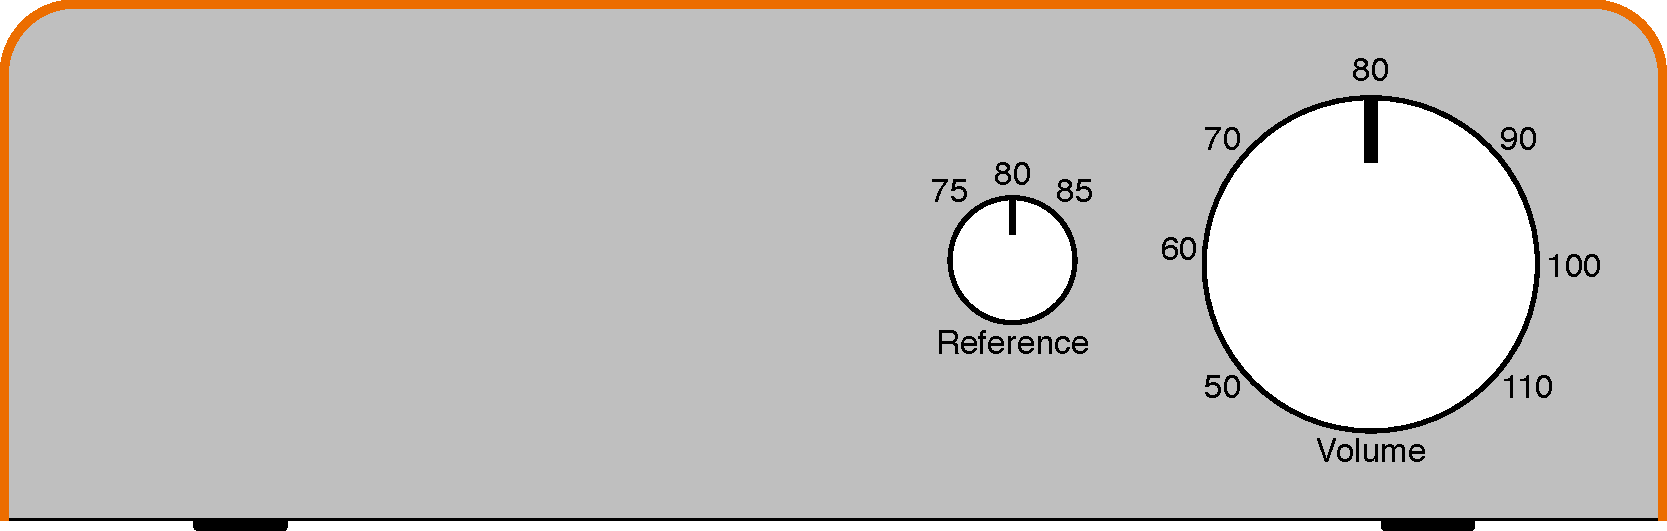
\includegraphics[resolution=300,width=\textwidth]{InterfaceFront}
	\caption{Koncepttegning af produktets forside med referenceindstilling og volumenkontrol}
	\label{fig:InterfaceFront}
\end{figure}
\noindent
Produktets forside består, venstre mod højre, af en drejeknap til indstilling af referencespænding og en drejeknap til volumenkontrol. Volumenkontrollens størrelse indikerer at det er den primære interaktion.\\
På produktets bagside placeres tilkoblingsmulighederne og bypass-funktionen.
\begin{figure}[H]
	\centering
	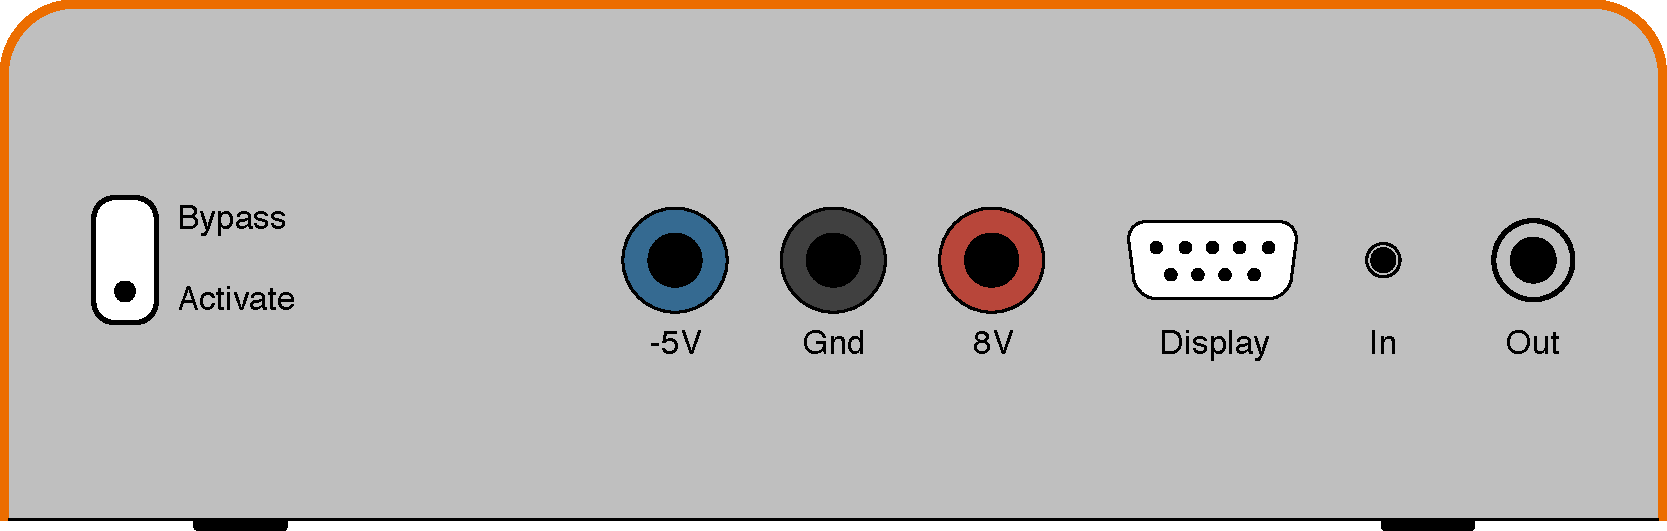
\includegraphics[resolution=300,width=\textwidth]{InterfaceBack}
	\caption{Koncepttegning af produktets bagside med mulighederne for at bypasse systemet, tilslutte en strømforsyning, display og sende lyd ind og ud.}
	\label{fig:InterfaceBack}
\end{figure}
\noindent
Produktets bagside består, venstre mod højre, af en knap til at bypasse systemet, stik til strømforsyning, stik til display og stik til lyd ind og ud.
%
\newpage
\noindent
%
På \autoref{fig:ProductScewFront} og \autoref{fig:ProductScewBack} repræsenteres det færdige produkt.
\begin{figure}[H]
	\centering
	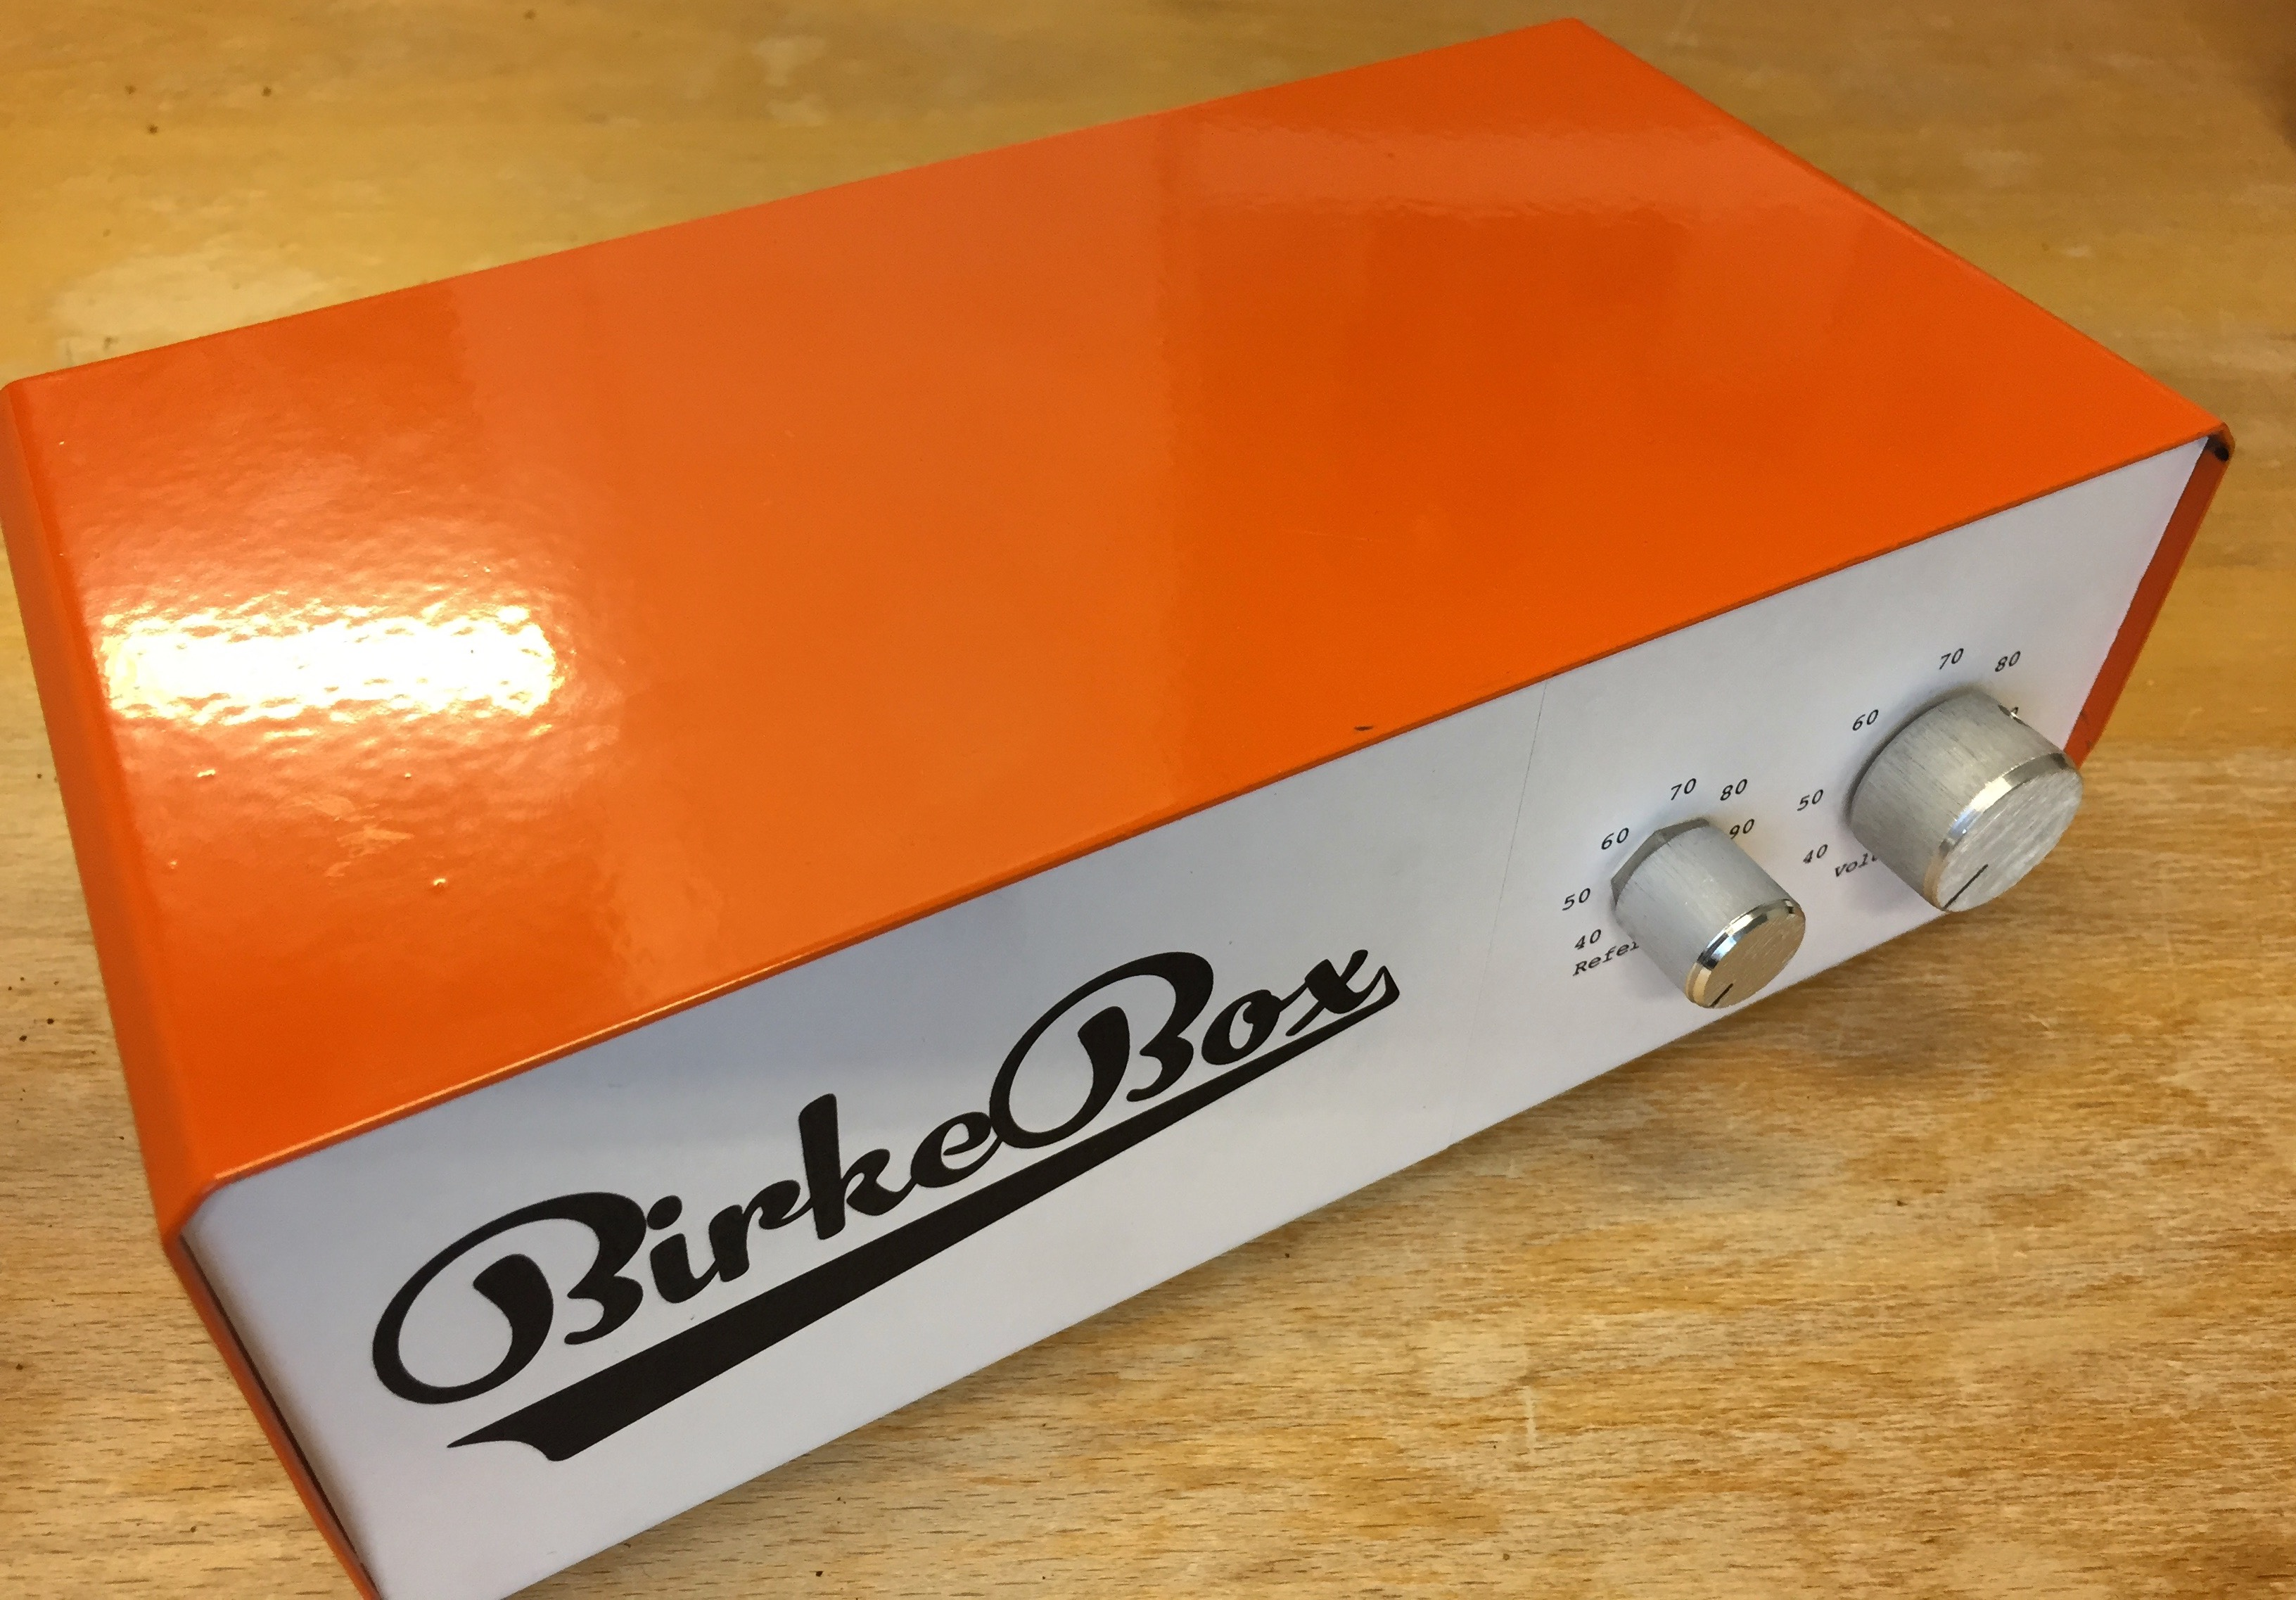
\includegraphics[resolution=300,width=\textwidth]{ProductShots/ProductScewFront}
	\caption{Det færdige produkt, set forfra}
	\label{fig:ProductScewFront}
\end{figure}
%
\noindent
\begin{figure}[H]
	\centering
	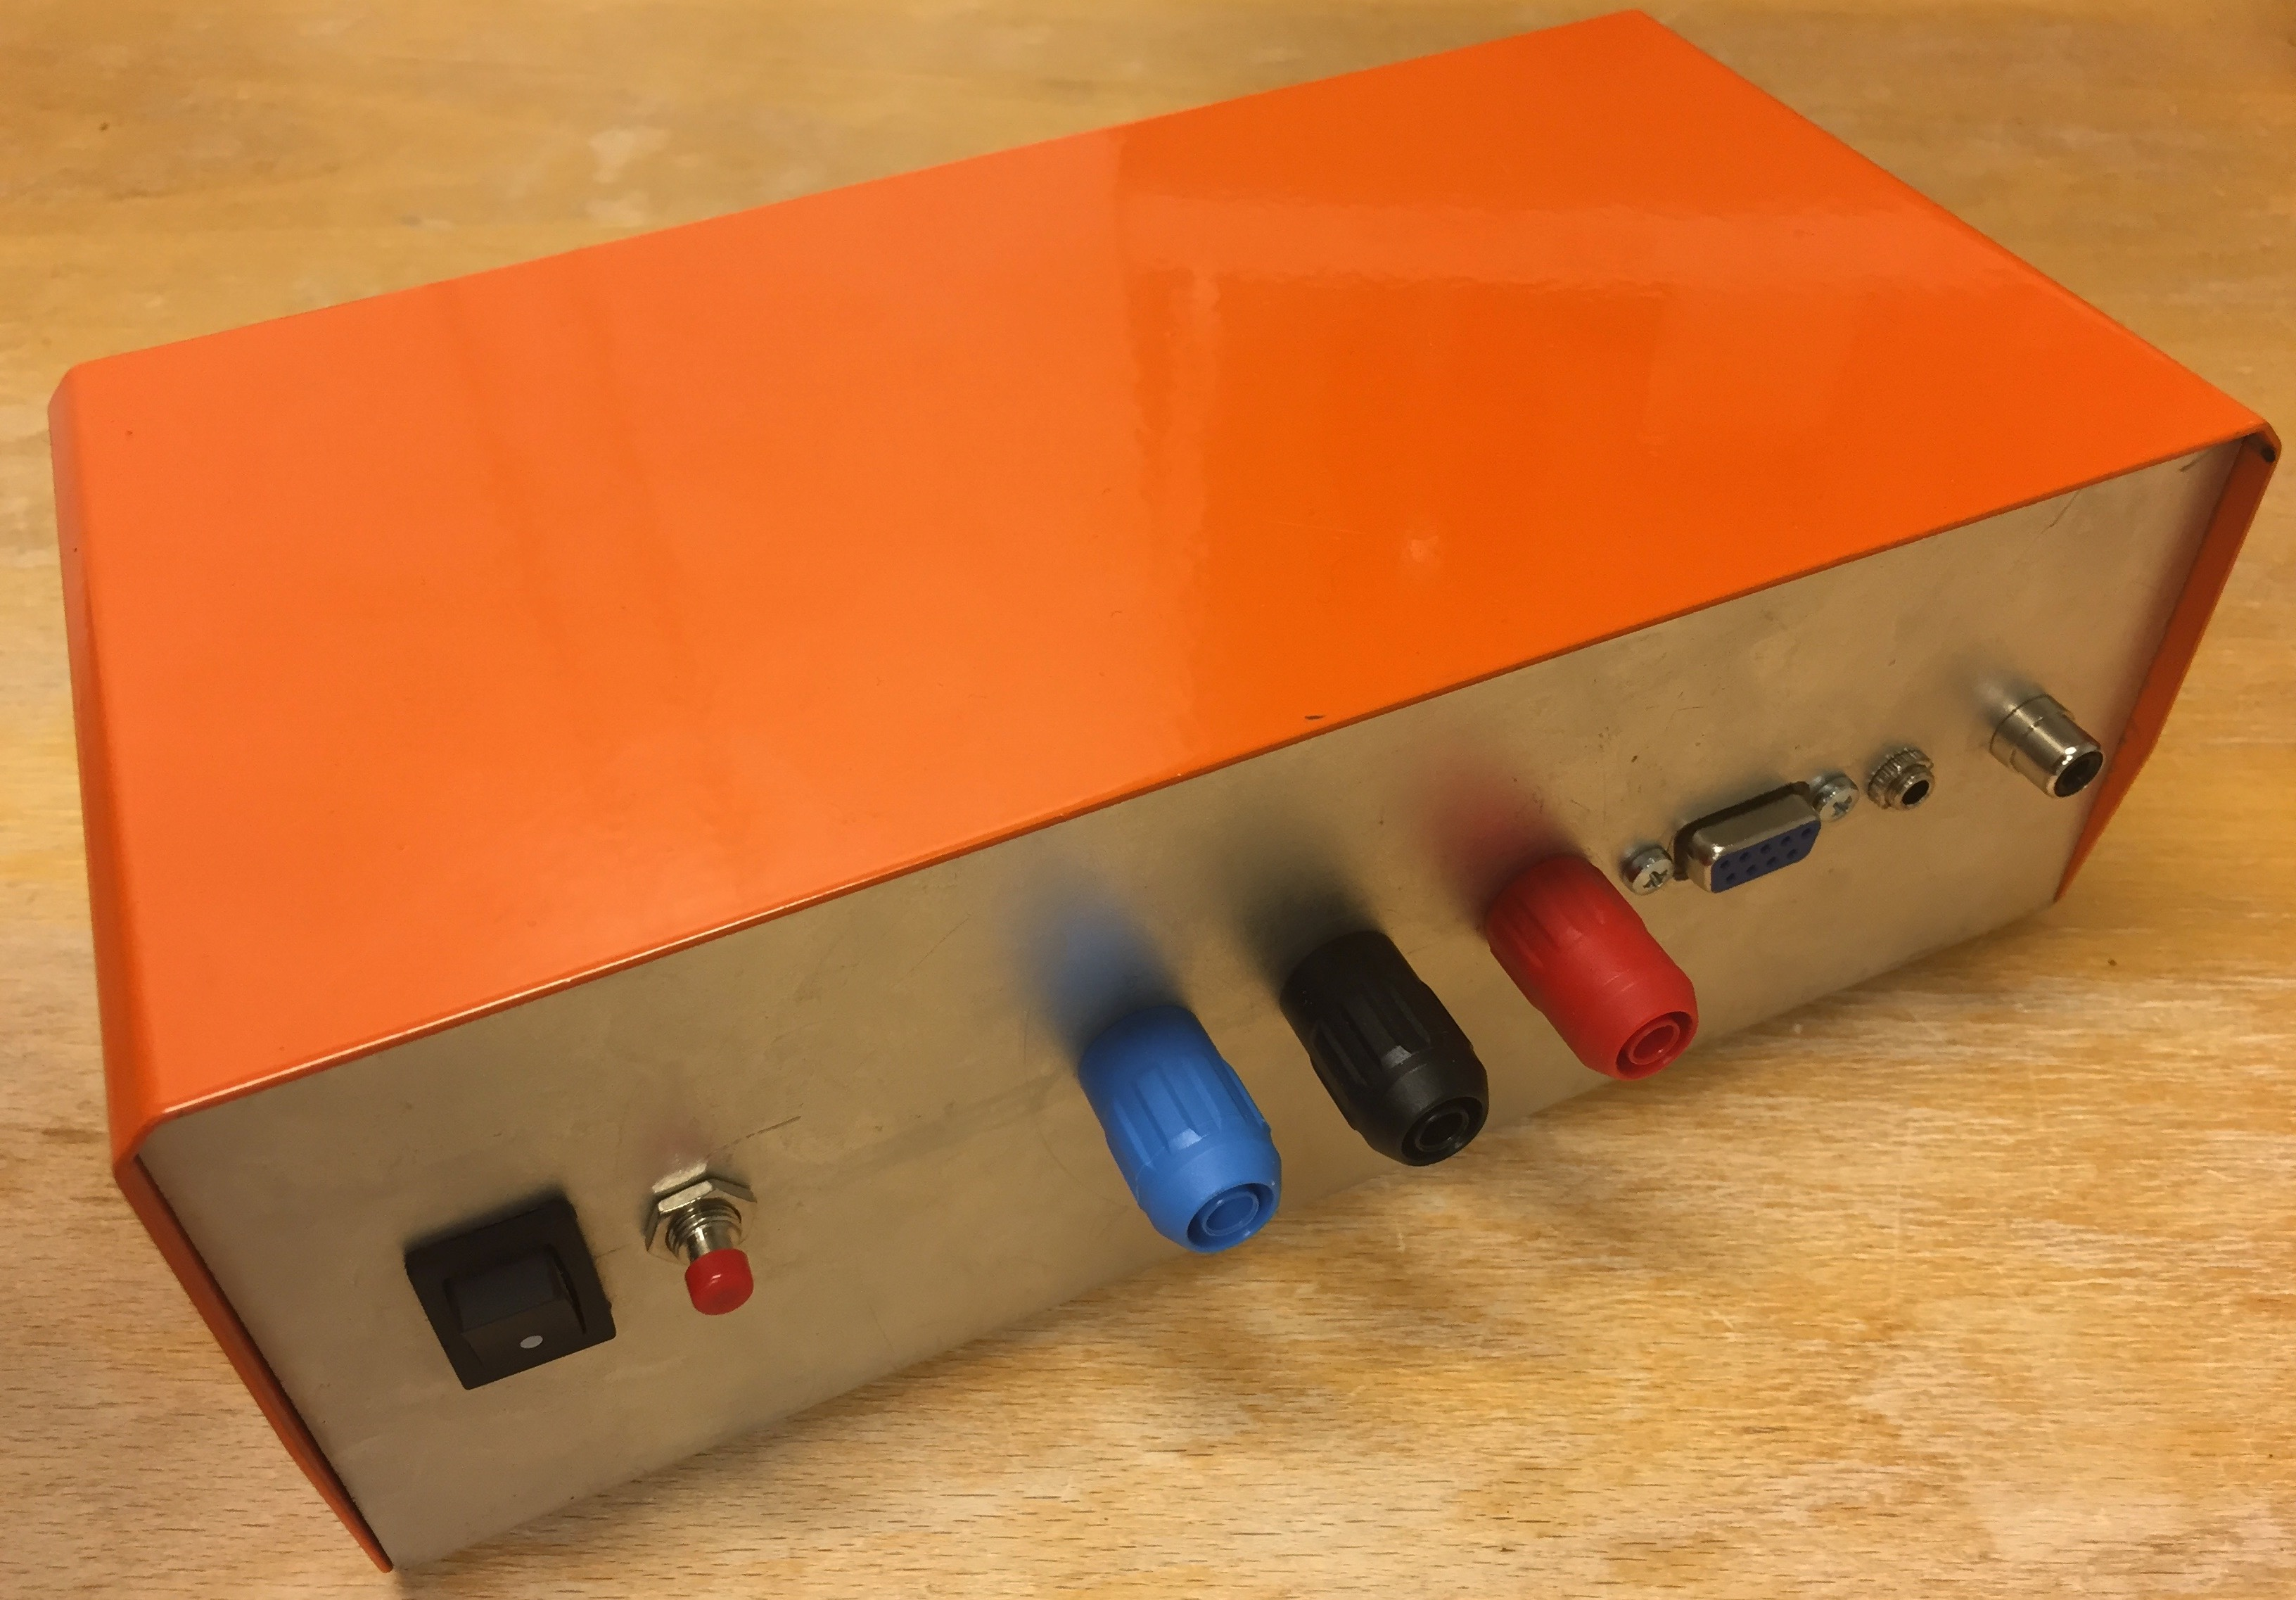
\includegraphics[resolution=300,width=\textwidth]{ProductShots/ProductScewBack}
	\caption{Det færdige produkt, set bagfra}
	\label{fig:ProductScewBack}
\end{figure}
\noindent
%
\newpage
\noindent
%
Displayet til fejlfinding er repræsenteret på \autoref{fig:Display}. Den gule LED længst til venstre lyser hvis et dæmpende filter er i brug, og er slukket, hvis det er et forstærkende filter, og afhænger af outputtet fra komparatoren, jævnfør \fullref{Komparator}. De fire grønne LED'er modtager et binært tal, som indikerer hvilket filter der aktiveres.
\begin{figure}[H]
	\centering
	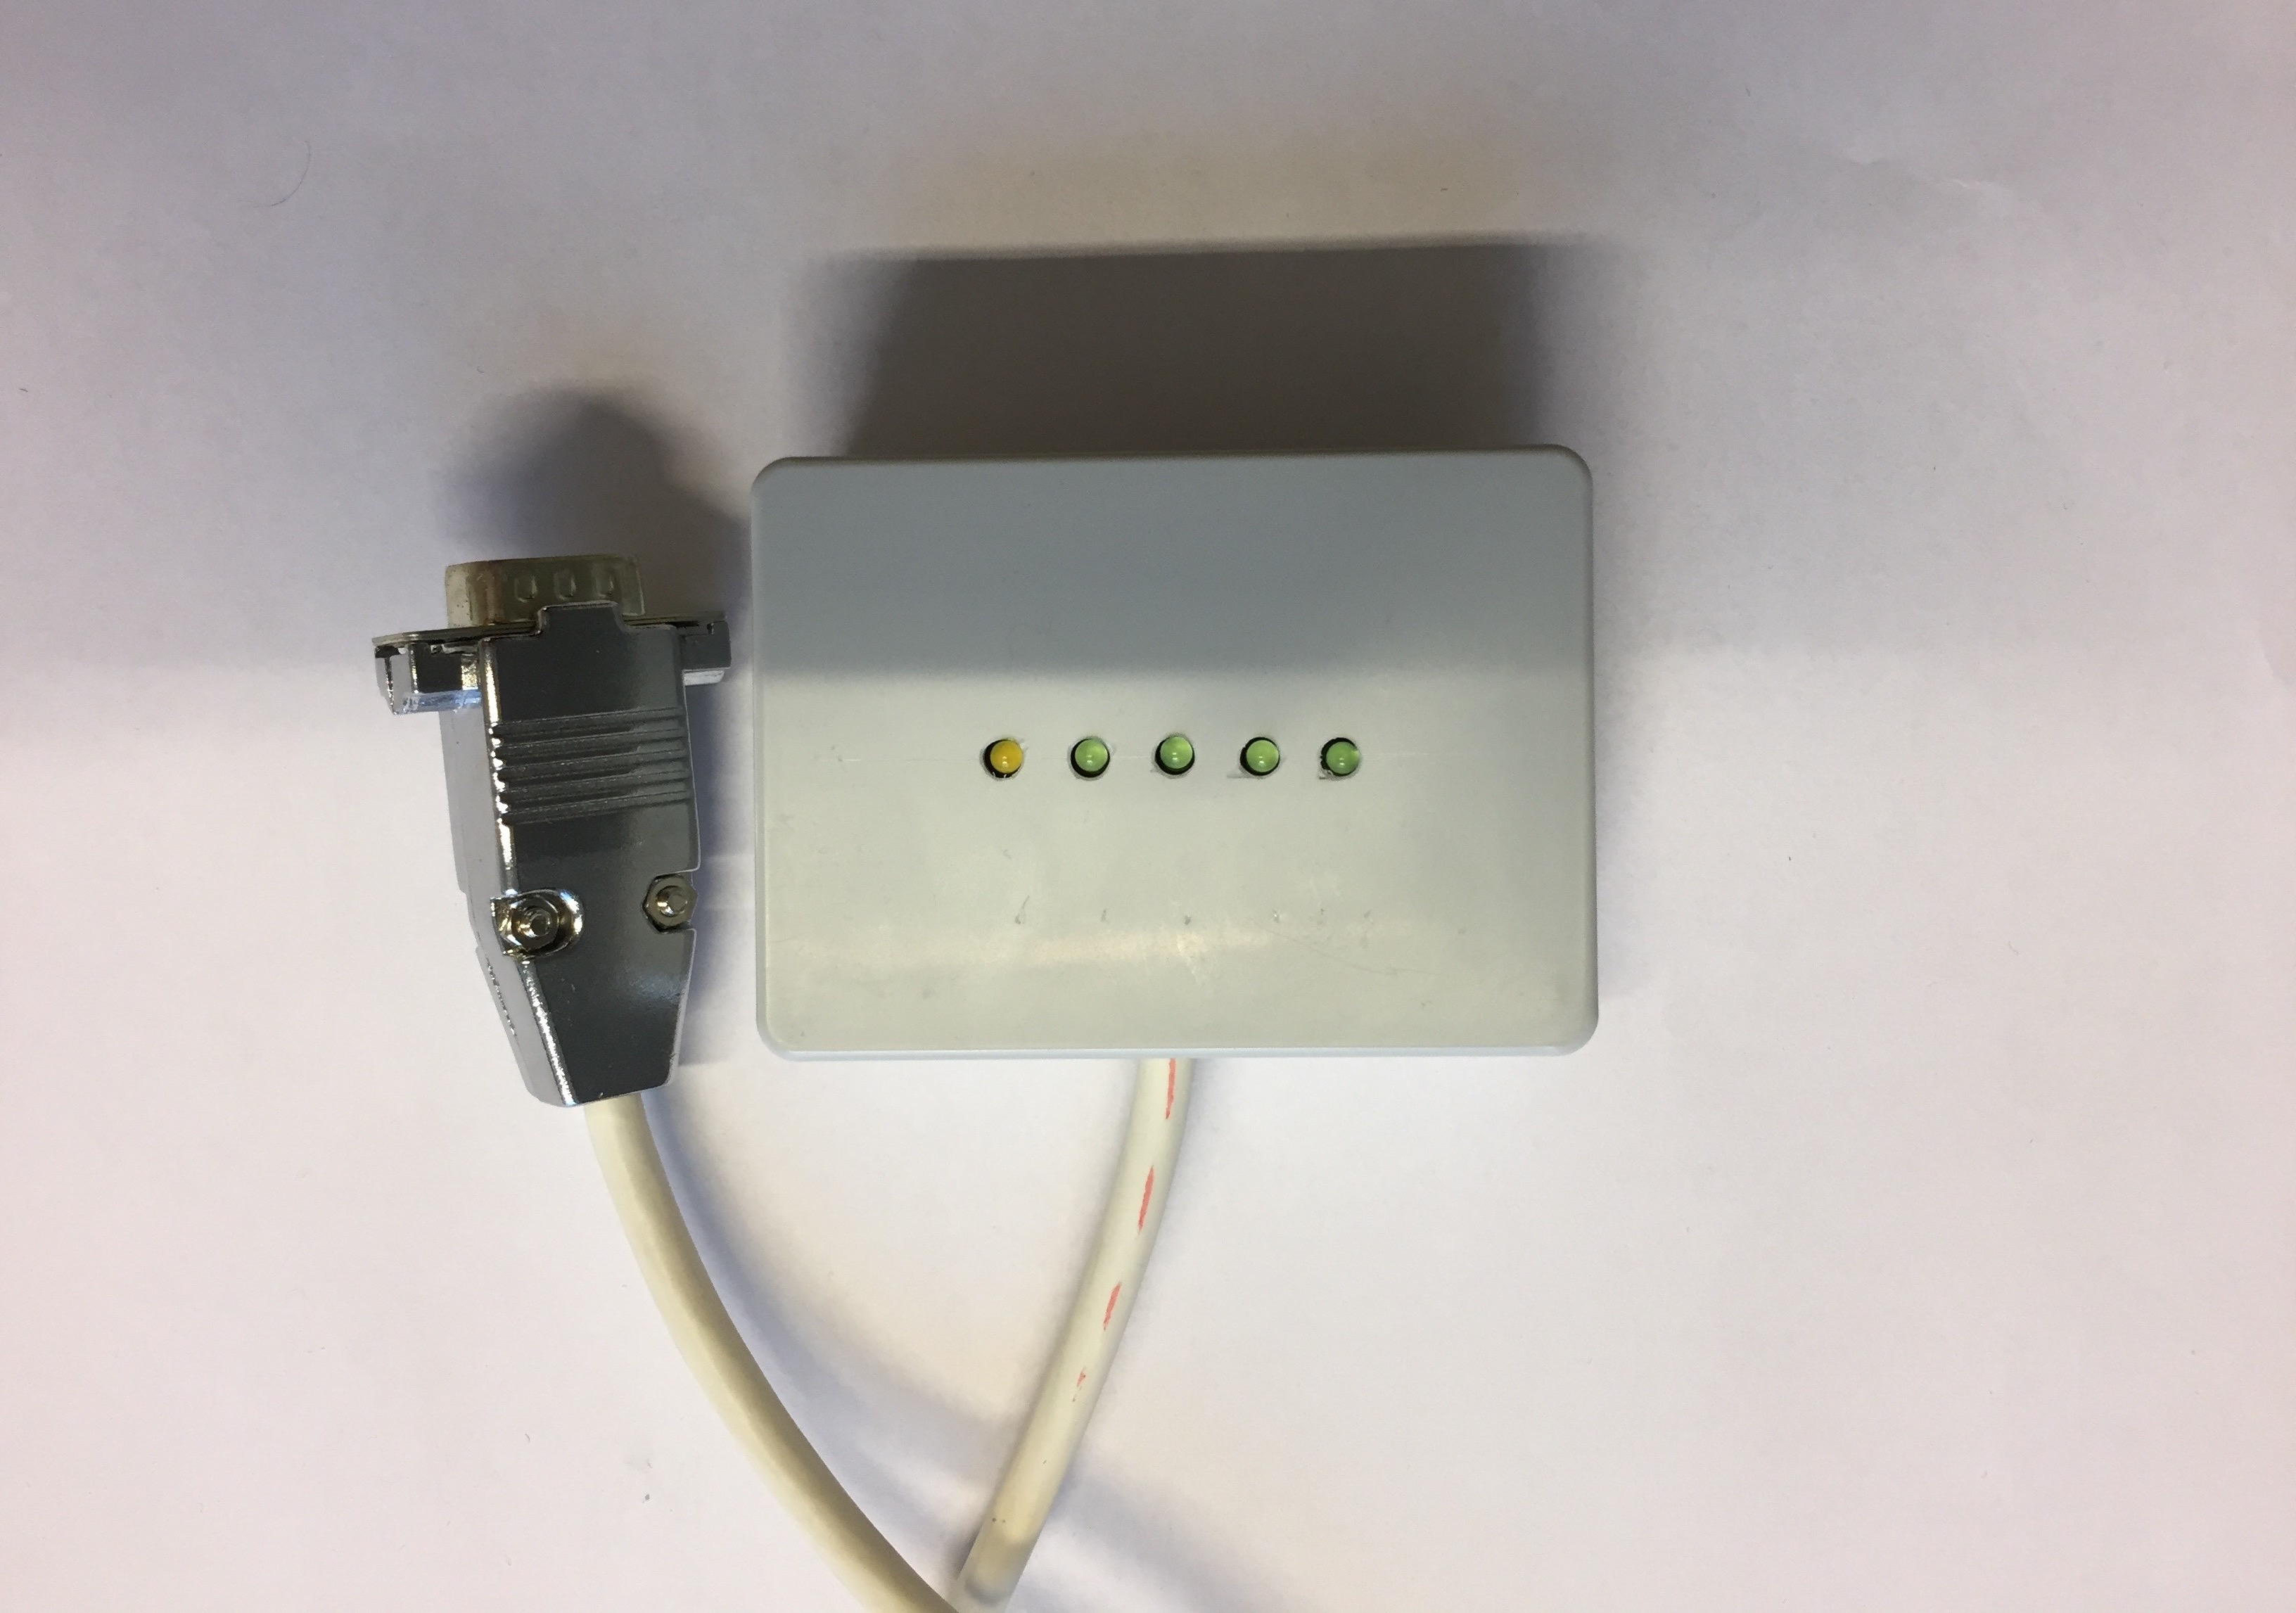
\includegraphics[resolution=300,width=\textwidth]{ProductShots/Display}
	\caption{Display til fejlfinding}
	\label{fig:Display}
\end{figure}
\noindent